\documentclass[10pt,a4paper]{article}
\usepackage[margin=1.5cm, top=1.3cm, bottom=1.3cm]{geometry}
\usepackage{graphicx}
\usepackage{booktabs}
\usepackage{array}
\usepackage{xcolor}
\usepackage{hyperref}
\usepackage{tikz}
\usepackage{tabularx}
\usepackage{enumitem}
\usepackage{multicol}
\usepackage{float}
\usepackage{parskip}
\setlength{\parskip}{2pt plus 1pt minus 1pt}
\setlength{\tabcolsep}{4pt}

\usetikzlibrary{shapes.geometric, arrows.meta, positioning, fit}

\definecolor{primary}{HTML}{1a1a2e}
\definecolor{accent}{HTML}{e94560}
\definecolor{secondary}{HTML}{0f3460}
\definecolor{darkgreen}{HTML}{2d6a4f}
\definecolor{darkorange}{HTML}{e76f51}

\hypersetup{colorlinks=true, linkcolor=secondary, urlcolor=accent}

\pagestyle{empty}

\begin{document}

% ============================================================
% PAGE 1
% ============================================================

\begin{center}
{\Huge\bfseries\textcolor{primary}{The Factory}}\\[0.3cm]
{\Large\textcolor{secondary}{Executive Brief --- February 2026}}\\[0.2cm]
{\small Prepared by the Kev Agent Team}
\end{center}

\vspace{0.2cm}
\rule{\textwidth}{1.5pt}
\vspace{0.1cm}

\section*{What Is It?}

An \textbf{autonomous AI factory} that discovers market opportunities, builds software products, deploys them, and generates revenue---24/7. Adam is the portfolio manager, not the operator. Four AI agents (Kev, Rex, Scout, Blaze) handle everything from market research to code deployment.

\section*{Key Numbers}

\begin{table}[H]
\centering
\begin{tabular}{lrl}
\toprule
\textbf{Metric} & \textbf{Value} & \textbf{Notes} \\
\midrule
12-month revenue target & \$30K--70K/mo & From 8--15 live products \\
Monthly cost (Month 1) & \$800--1,000 & LLM APIs + electricity + hosting \\
Monthly cost (Month 12) & \$6,500--7,300 & At full operation \\
Break-even & Month 5--7 & Conservative estimate \\
Infrastructure services & 5 & On a single 64GB RAM server \\
Cost per product built & \$40--70 & Full cycle: research to deployment \\
Time to build a product & 15--25 min & Agent time (excl. human approval) \\
\bottomrule
\end{tabular}
\end{table}

\section*{Architecture}

\begin{center}
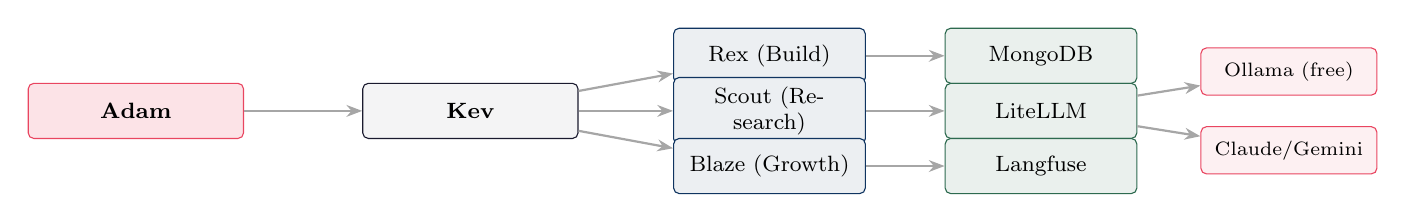
\begin{tikzpicture}[
    node distance=0.8cm and 1.5cm,
    box/.style={rectangle, draw=secondary, fill=secondary!8, text width=2.2cm, minimum height=0.7cm, align=center, rounded corners=2pt, font=\footnotesize},
    bigbox/.style={rectangle, draw=primary, fill=primary!5, text width=2.5cm, minimum height=0.7cm, align=center, rounded corners=2pt, font=\footnotesize\bfseries},
    cloud/.style={rectangle, draw=accent, fill=accent!8, text width=2cm, minimum height=0.6cm, align=center, rounded corners=2pt, font=\scriptsize},
    arr/.style={-{Stealth[length=2mm]}, thick, color=gray!70}
]

\node[bigbox, fill=accent!15, draw=accent] (adam) {Adam};
\node[bigbox, right=of adam] (kev) {Kev};
\node[box, right=1.2cm of kev, yshift=0.7cm] (rex) {Rex (Build)};
\node[box, right=1.2cm of kev] (scout) {Scout (Research)};
\node[box, right=1.2cm of kev, yshift=-0.7cm] (blaze) {Blaze (Growth)};

\node[box, right=1cm of rex, fill=darkgreen!10, draw=darkgreen] (mongo) {MongoDB};
\node[box, right=1cm of scout, fill=darkgreen!10, draw=darkgreen] (litellm) {LiteLLM};
\node[box, right=1cm of blaze, fill=darkgreen!10, draw=darkgreen] (langfuse) {Langfuse};

\node[cloud, right=0.8cm of litellm, yshift=0.5cm] (local) {Ollama (free)};
\node[cloud, right=0.8cm of litellm, yshift=-0.5cm] (cloud) {Claude/Gemini};

\draw[arr] (adam) -- (kev);
\draw[arr] (kev) -- (rex);
\draw[arr] (kev) -- (scout);
\draw[arr] (kev) -- (blaze);
\draw[arr] (rex) -- (mongo);
\draw[arr] (scout) -- (litellm);
\draw[arr] (blaze) -- (langfuse);
\draw[arr] (litellm) -- (local);
\draw[arr] (litellm) -- (cloud);

\end{tikzpicture}
\end{center}

\section*{The Pipeline}

\begin{center}
\textbf{SCAN} $\xrightarrow{\text{Scout}}$ \textbf{VALIDATE} $\xrightarrow{\text{Scout}}$ \textbf{BUILD} $\xrightarrow{\text{Rex}}$ \textbf{LAUNCH} $\xrightarrow{\text{Rex}}$ \textbf{GROW} $\xrightarrow{\text{Blaze}}$
\end{center}

2--5 days per product. Launch 2/month, 30\% survive, survivors avg \$2K/month by month 6.

\newpage

% ============================================================
% PAGE 2
% ============================================================

\section*{Technology Stack}

\begin{table}[H]
\centering
\small
\begin{tabularx}{\textwidth}{llX}
\toprule
\textbf{Component} & \textbf{Choice} & \textbf{Why} \\
\midrule
Database & MongoDB & Replaces 7 systems: task queue, vector search, metrics, events, graph, cache, message bus \\
LLM Gateway & LiteLLM & 100+ providers, per-key budgets, fallback chains, cost logging \\
LLM Execution & Pi SDK & Spawns parallel Claude Code/Codex sessions \\
Observability & Langfuse & Per-trace cost tracking; native LiteLLM integration \\
Language & TypeScript & Ecosystem alignment; products + factory in one language \\
Products Deploy & Cloudflare & 100K req/day free; zero cold starts; global edge \\
Auth / Payments & Clerk + Stripe & Free tiers; industry standard; agent-friendly \\
Local Inference & Ollama (RTX 3090) & 50--60\% of calls free; embeddings always local \\
\bottomrule
\end{tabularx}
\end{table}

\section*{First Product: CronPilot}

Cron job monitoring for developers. \$7--49/month. 97\% margin. 18 agent-hours to build. \$105--135 total cost to launch. Proven market (Cronitor is \$20M+), underserved at the indie price point.

\textbf{Build plan:} 3 days. Day 1: foundation + ping endpoint. Day 2: dashboard + billing. Day 3: QA + launch.

\section*{Week 1 Sprint Plan}

\begin{table}[H]
\centering
\small
\begin{tabularx}{\textwidth}{lX}
\toprule
\textbf{Day} & \textbf{Deliverables} \\
\midrule
Mon & MongoDB task store, state machine, task CLI \\
Tue & Kev routing engine, cost pyramid, agent registry \\
Wed & Scout$\rightarrow$Rex pipeline (first automated chain) \\
Thu & QA gate (cross-model review), review queue \\
Fri & Integration hardening, live demo with real product ideas \\
\bottomrule
\end{tabularx}
\end{table}

\textbf{Friday demo:} Idea $\rightarrow$ Scout researches $\rightarrow$ Rex builds $\rightarrow$ QA validates $\rightarrow$ review queue. All autonomous.

\section*{Top 5 Risks}

\begin{table}[H]
\centering
\small
\begin{tabularx}{\textwidth}{Xlp{5.5cm}}
\toprule
\textbf{Risk} & \textbf{Score} & \textbf{Key Mitigation} \\
\midrule
API cost blowout / runaway loops & 20 & Per-agent budget caps, kill switches, velocity alerts \\
Prompt injection & 20 & Dual-LLM pattern, tool allowlists, human gates \\
Single server failure & 16 & UPS, auto-restart, cloud fallback, git for code \\
Platform bans (Stripe) & 15 & Legitimate products, multiple processors, low chargebacks \\
No product-market fit & 15 & Validation before building, fast kill decisions, portfolio approach \\
\bottomrule
\end{tabularx}
\end{table}

\section*{Next Steps}

\begin{enumerate}[itemsep=2pt]
    \item \textbf{This week:} Execute Week 1 sprint --- task queue, routing, first pipeline
    \item \textbf{Week 2:} Deployment pipeline, first production ship
    \item \textbf{Week 3--4:} Approval flow, cost controls, CronPilot launch
    \item \textbf{Month 2:} Pipeline tuned, 2--3 products/week
    \item \textbf{Month 3:} Factory self-funding from product revenue
\end{enumerate}

\vfill
\begin{center}
\rule{0.5\textwidth}{0.4pt}\\[0.3cm]
{\small\textcolor{gray}{The Factory --- Executive Brief --- February 8, 2026}}
\end{center}

\end{document}
